\documentclass[14pt]{extarticle}
\usepackage[russian]{babel}
\usepackage[utf8]{inputenc}
\usepackage[T2A]{fontenc}
\usepackage{graphicx}
\usepackage[export]{adjustbox}
\usepackage{amsmath}
\usepackage{amsfonts}
\usepackage{amssymb}
\usepackage[version=4]{mhchem}
\usepackage{stmaryrd}

\usepackage[left=2cm, right=2cm, top=2cm, bottom=2cm]{geometry}


\usepackage{minted}
\usemintedstyle{vs}
% \usepackage{listings}
% \usepackage{xcolor}

% \definecolor{codegreen}{rgb}{0,0.6,0}
% \definecolor{codegray}{rgb}{0.5,0.5,0.5}
% \definecolor{codekey}{rgb}{0,0.4,1}
% \definecolor{codepurple}{rgb}{0.58,0,0.82}
% \definecolor{backcolour}{rgb}{0.95,0.95,0.95}

% \lstdefinestyle{mystyle}{
%     backgroundcolor=\color{backcolour},   
%     commentstyle=\color{codegreen},
%     keywordstyle=\color{codekey},
%     numberstyle=\tiny\color{codegray},
%     stringstyle=\color{codepurple},
%     basicstyle=\ttfamily\footnotesize,
%     breakatwhitespace=false,         
%     breaklines=true,                 
%     captionpos=b,                    
%     keepspaces=true,                 
%     numbers=left,                    
%     numbersep=5pt,                  
%     showspaces=false,                
%     showstringspaces=false,
%     showtabs=false,                  
%     tabsize=2
% }

% \lstset{style=mystyle}

\graphicspath{ {./images/} }


\title{Технология. Arduino \\ 8 класс 255 школа \\
 Методическое пособие}

\author{Ярмолинский Арсений Маркович}
\date{10 сентября 2024 г. }

\begin{document}
\maketitle
\tableofcontents

\graphicspath{{intro/images}}

\newcommand{\maxwidth}{\textwidth}
\newcommand{\maxheight}{0.44\textheight}
\newcommand{\maxlessheight}{0.35\textheight}

\section{Начало работы в WokWi}

\subsection{Создание проекта}

\begin{enumerate}

    \item Вид главной страницы Wokwi:
    
    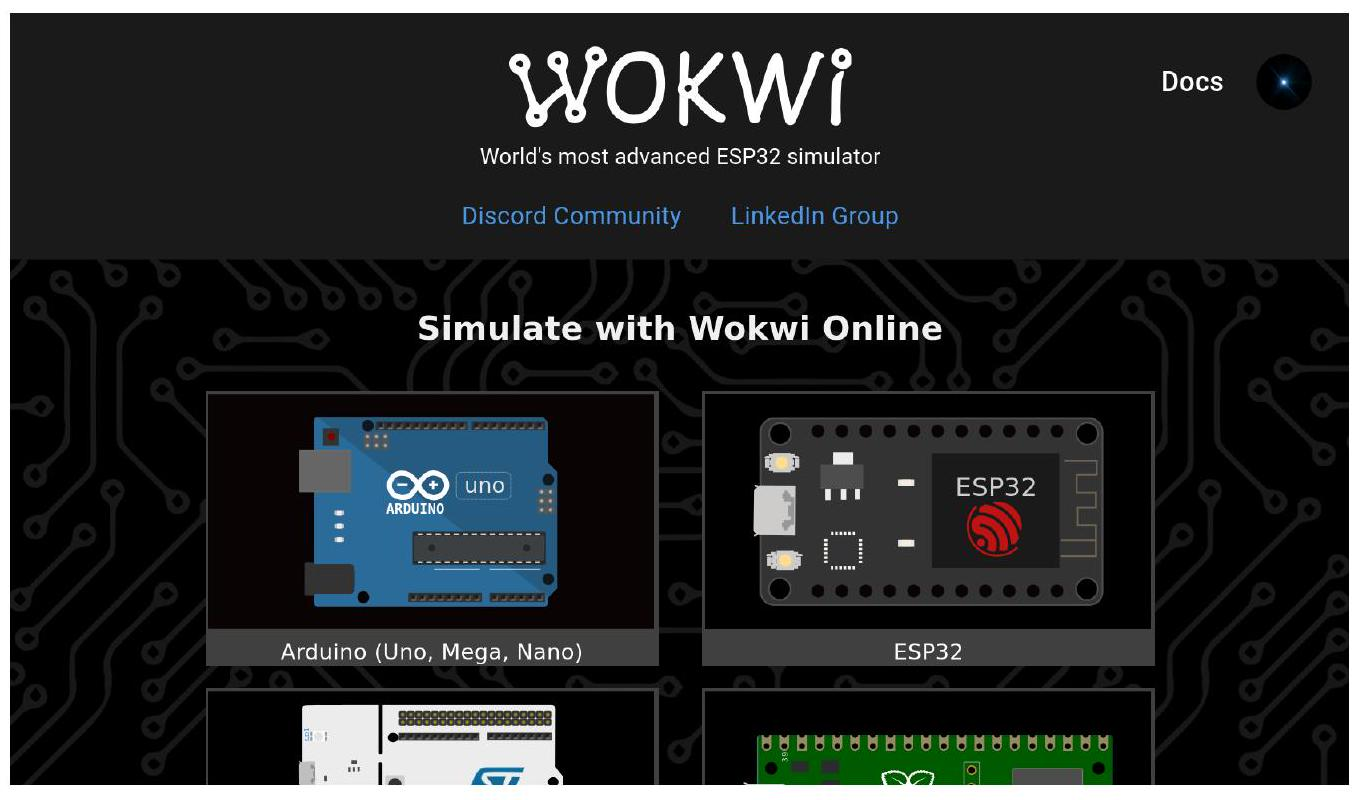
\includegraphics[max width=\maxwidth, max height=\maxlessheight, center]{1.jpg}    
    
    \item Откройте выпадающее меню профиля и нажмите кнопку "Мои проекты"\\
    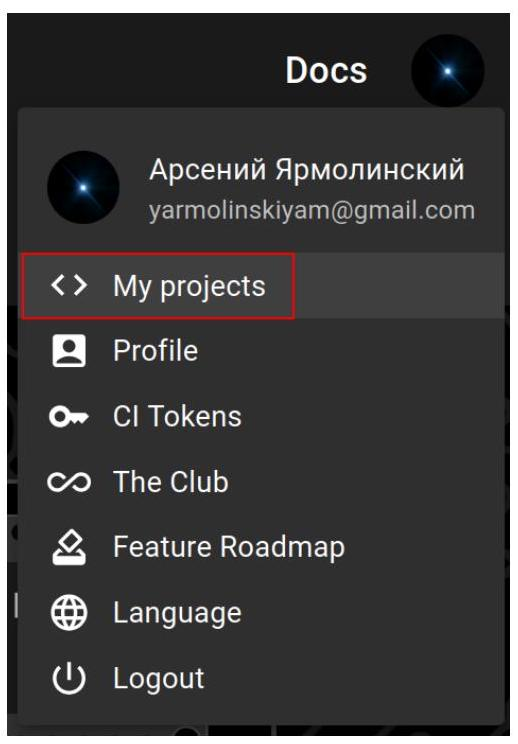
\includegraphics[max width=\maxwidth, max height=\maxheight, center]{2}
    
    \clearpage\item Страница проектов\\
    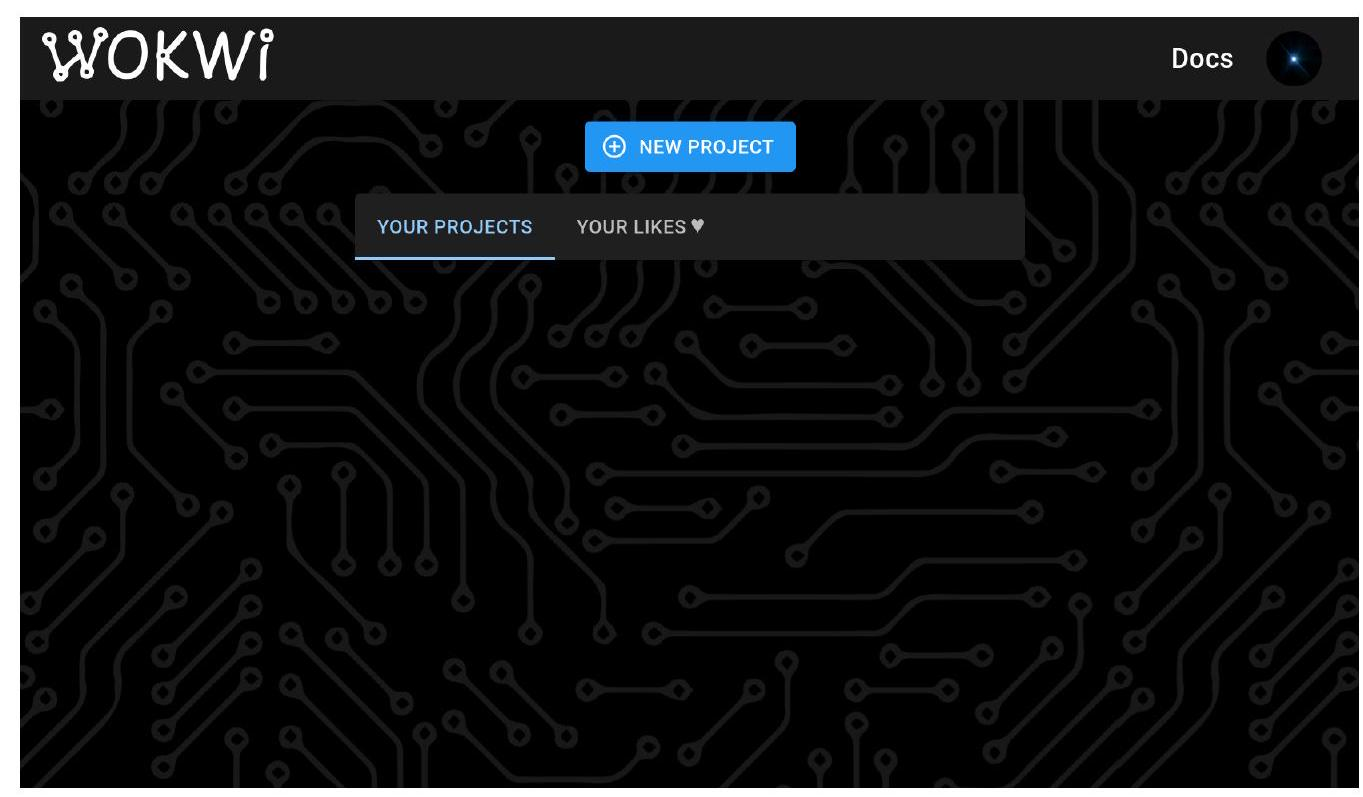
\includegraphics[max width=\maxwidth, max height=\maxheight, center]{3}
    
    \item Создайте новый проект\\
    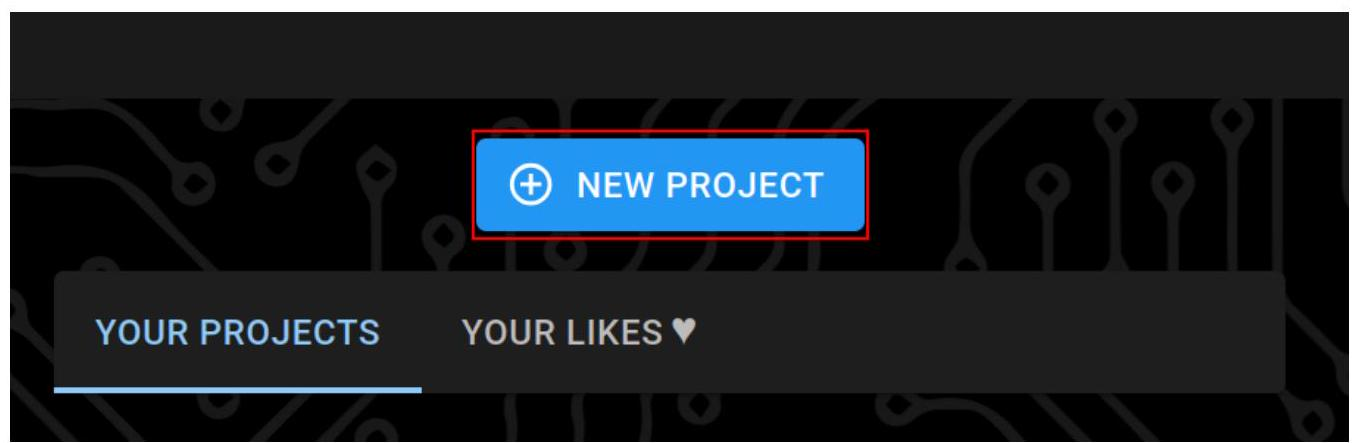
\includegraphics[max width=\maxwidth, max height=\maxheight, center]{4}
    
    \clearpage\item Выберите в меню слева семейство контроллеров Arduino\\
    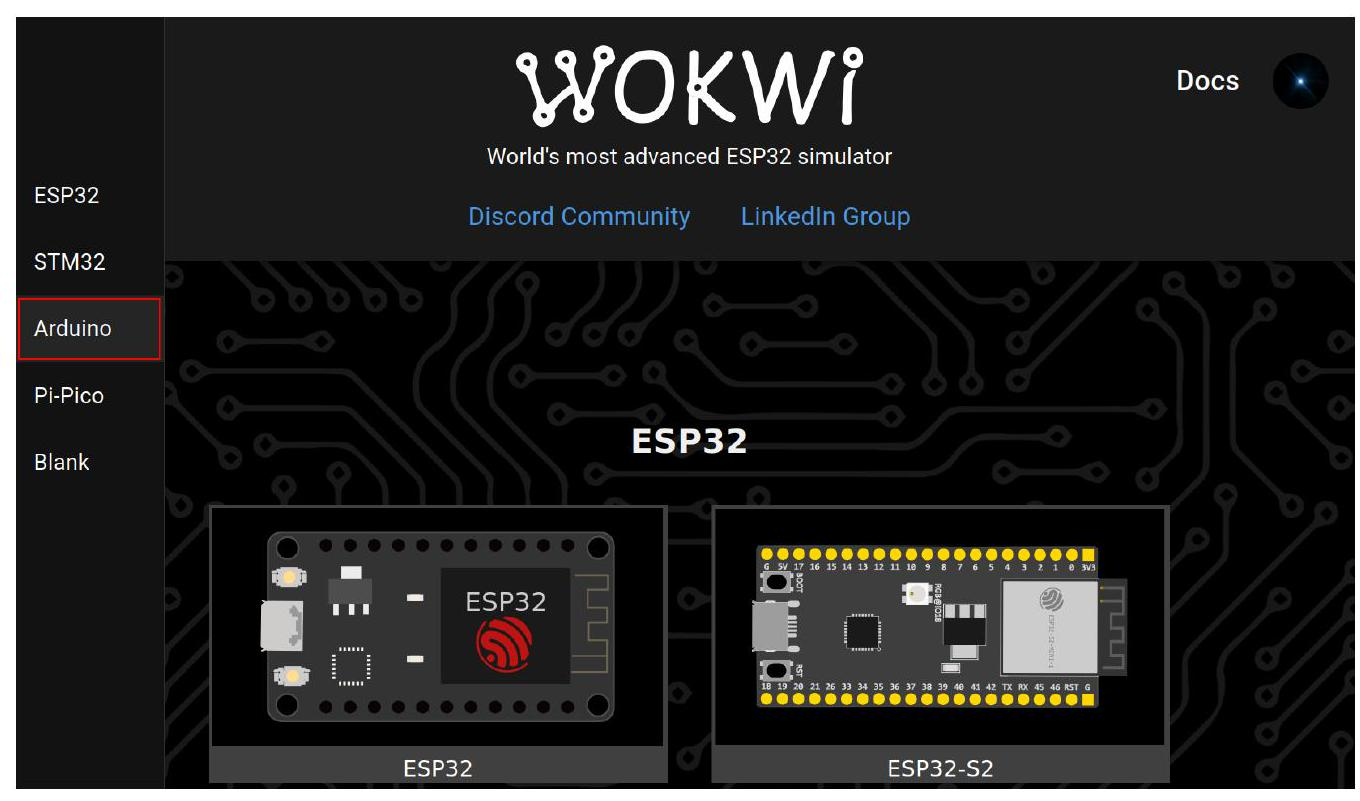
\includegraphics[max width=\maxwidth, max height=\maxheight, center]{5}
    
    \item Выберите контроллер Arduino Uno Rev3\\
    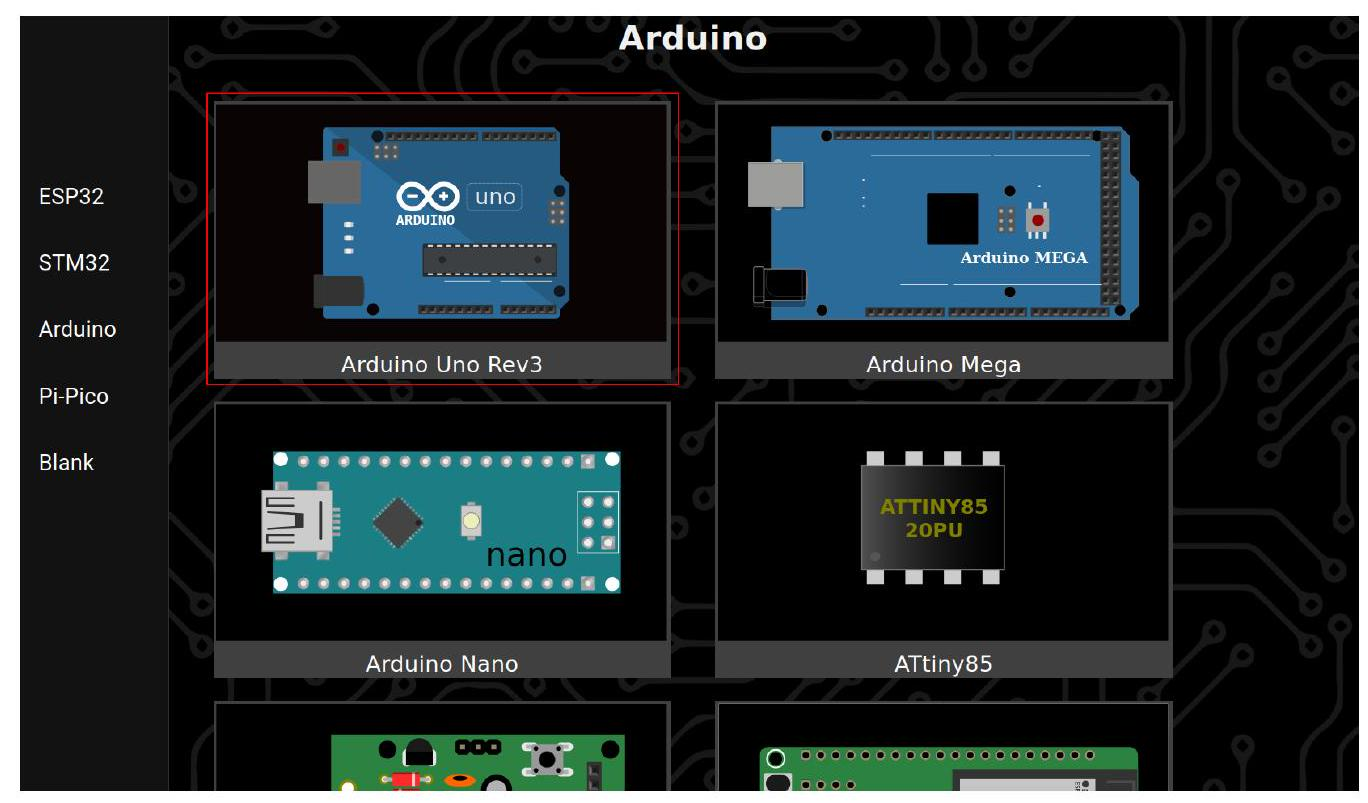
\includegraphics[max width=\maxwidth, max height=\maxheight, center]{6}

    \clearpage\item Созданный пустой проект!\\
    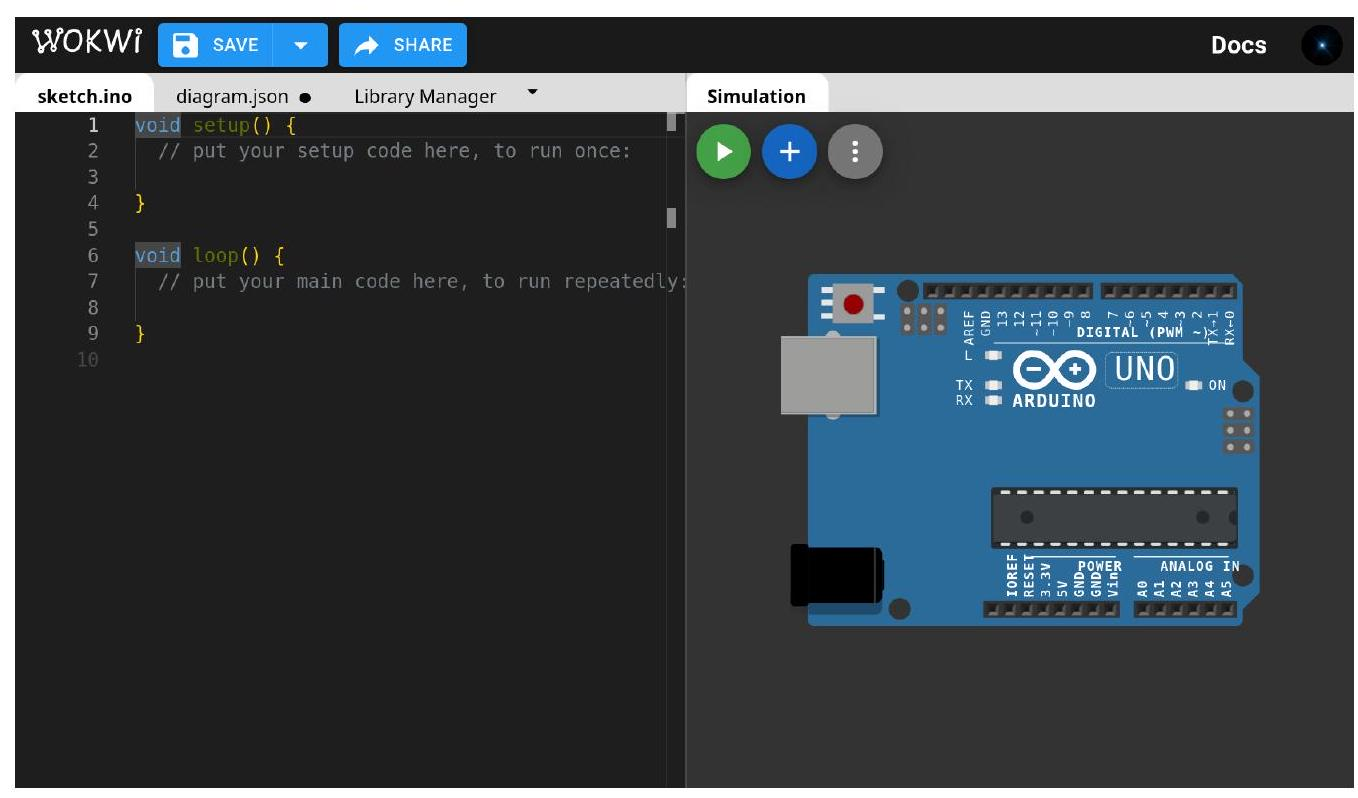
\includegraphics[max width=\maxwidth, max height=\maxheight, center]{7}

    \item После внесения изменений сохраните проект с помощью кнопки SAVE\\
    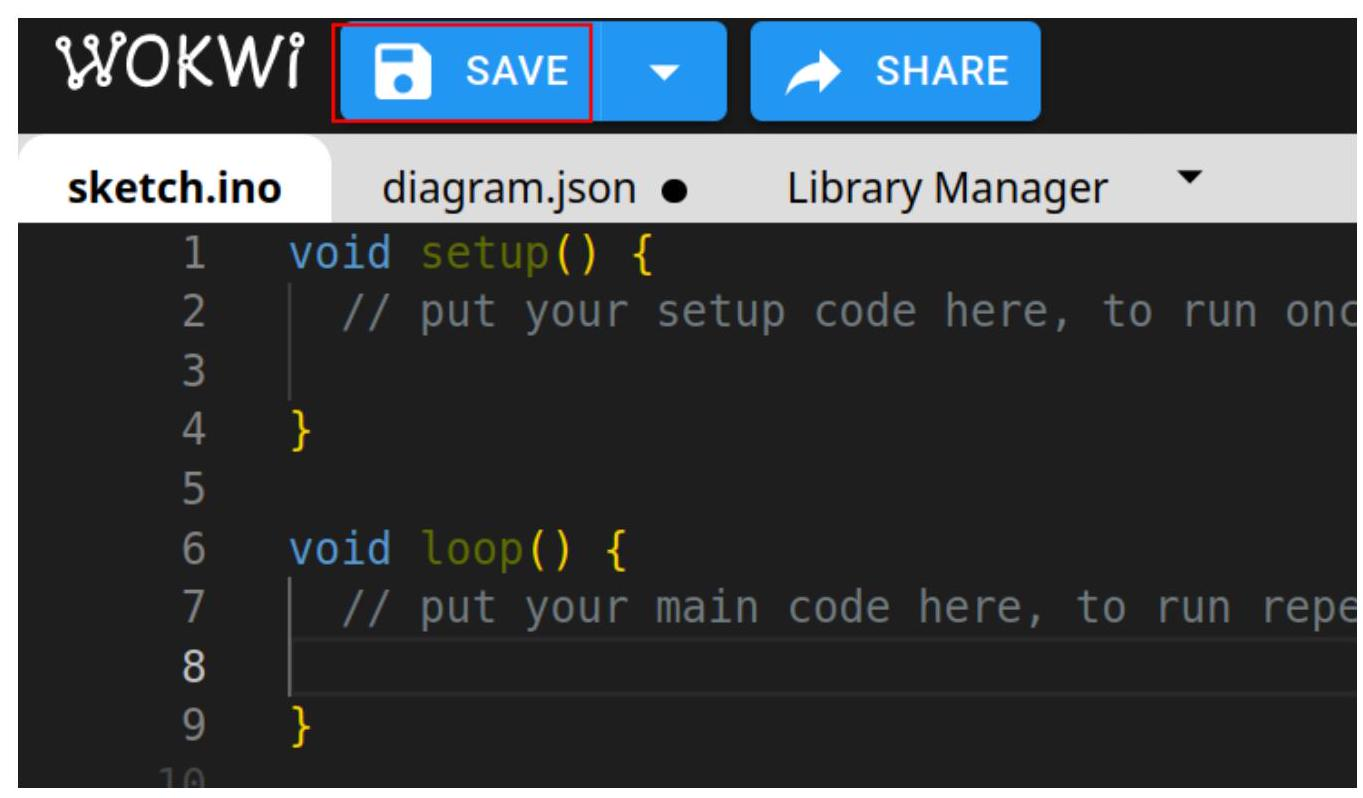
\includegraphics[max width=\maxwidth, max height=\maxheight, center]{8}

    \clearpage\item Введите название проекта и убедитесь, что он сохраняется как Public\\
    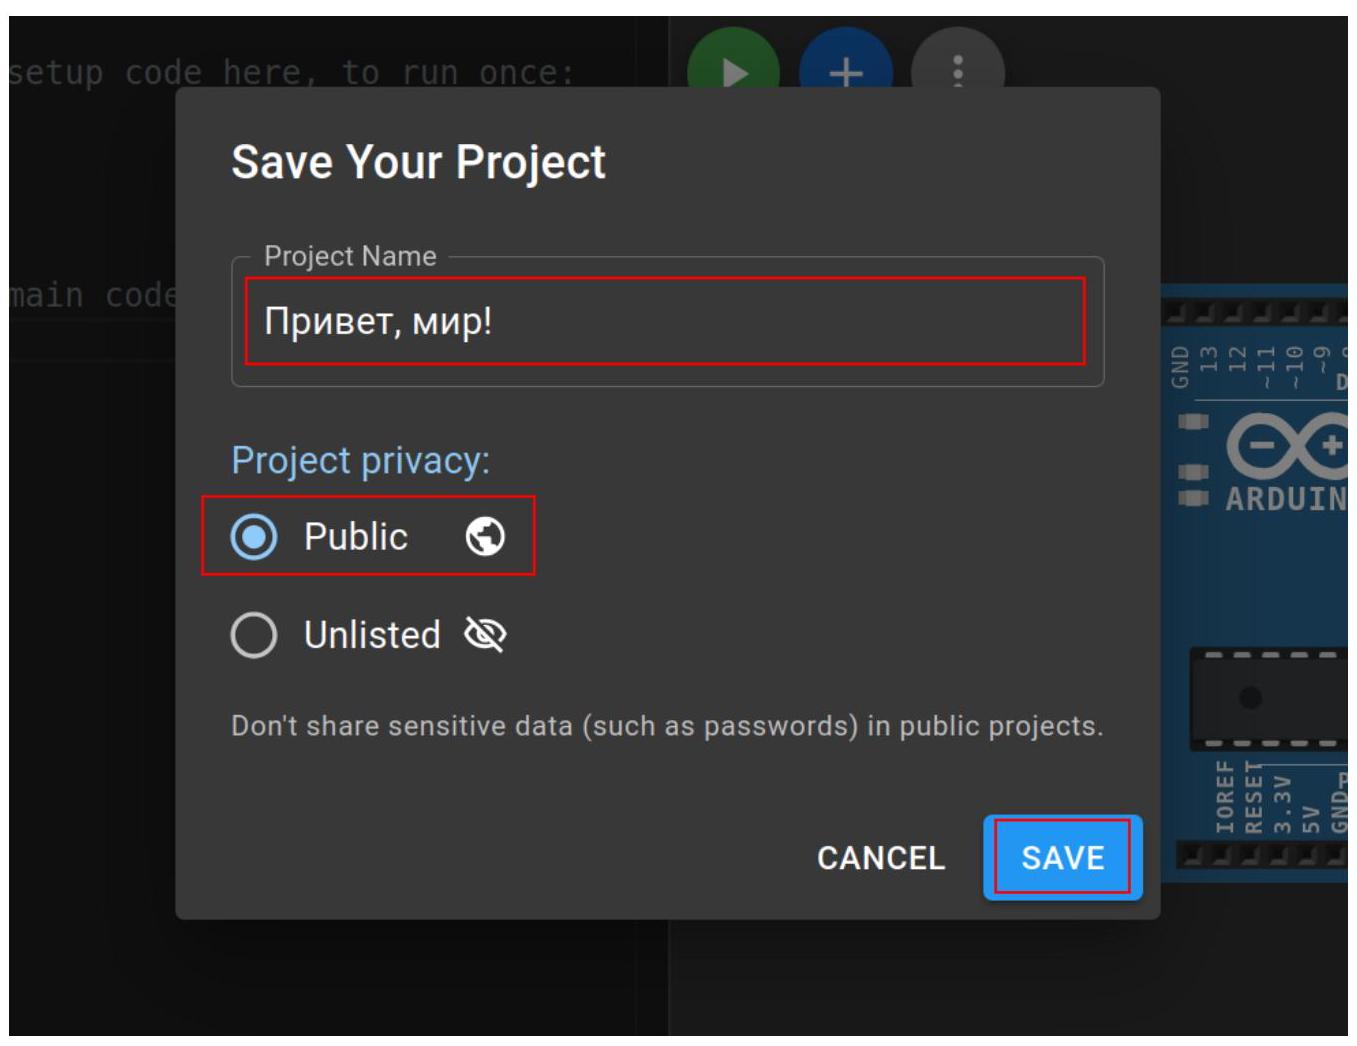
\includegraphics[max width=\maxwidth, max height=\maxheight, center]{9}

    \item Для добавления новой детали нажмите кнопку добавления\\
    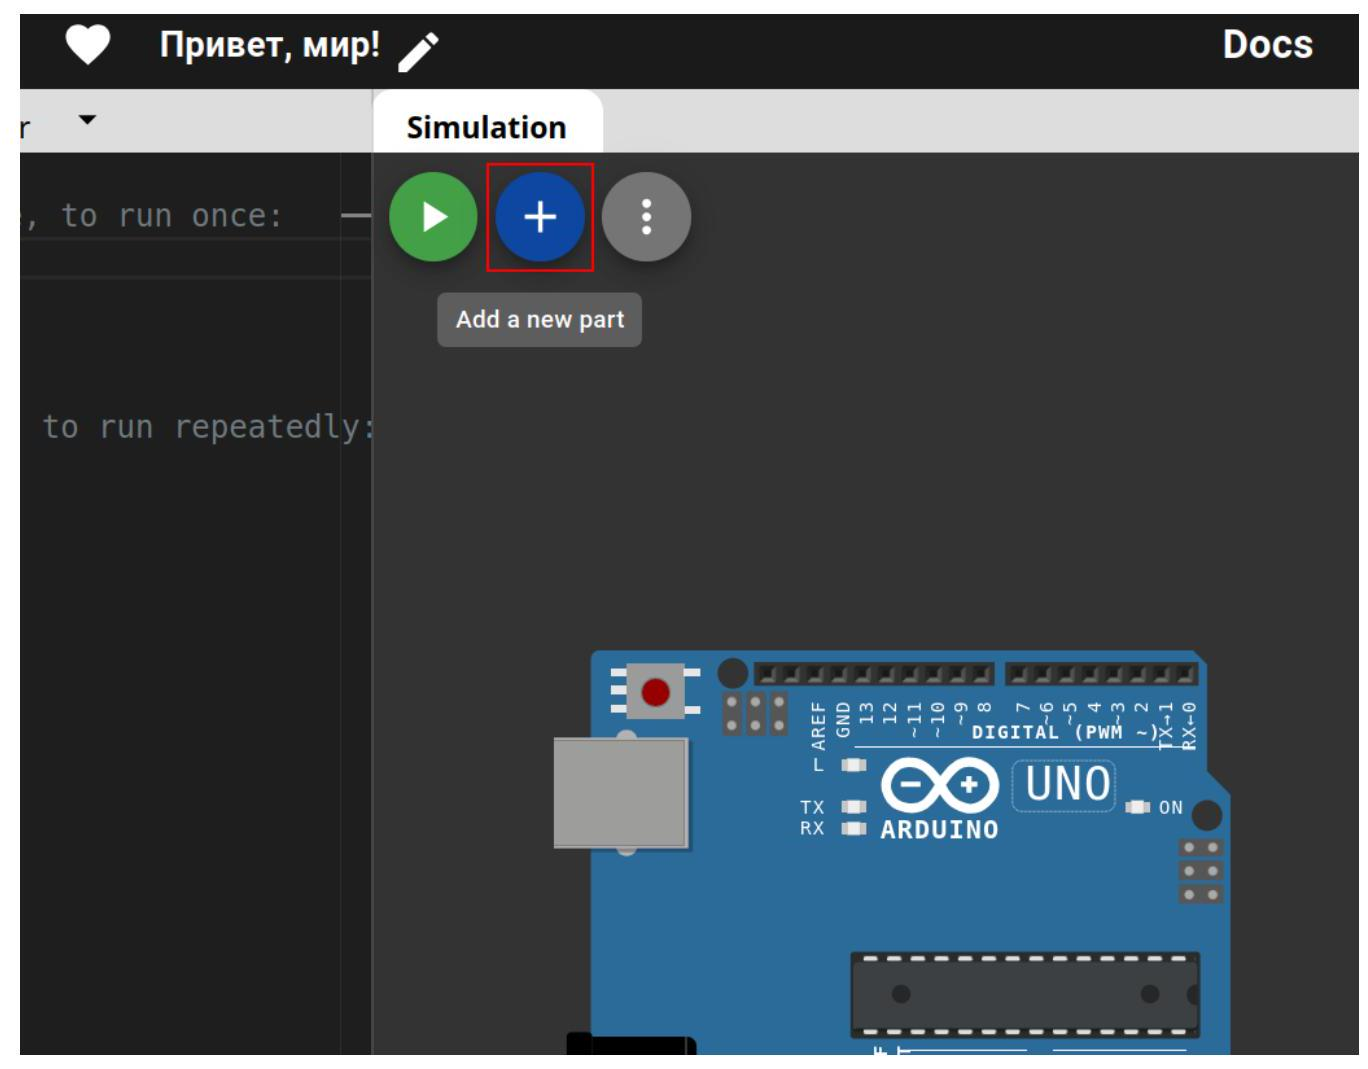
\includegraphics[max width=\maxwidth, max height=\maxheight, center]{10}

    \clearpage\item И выберите нужную деталь из выпадающего меню\\
    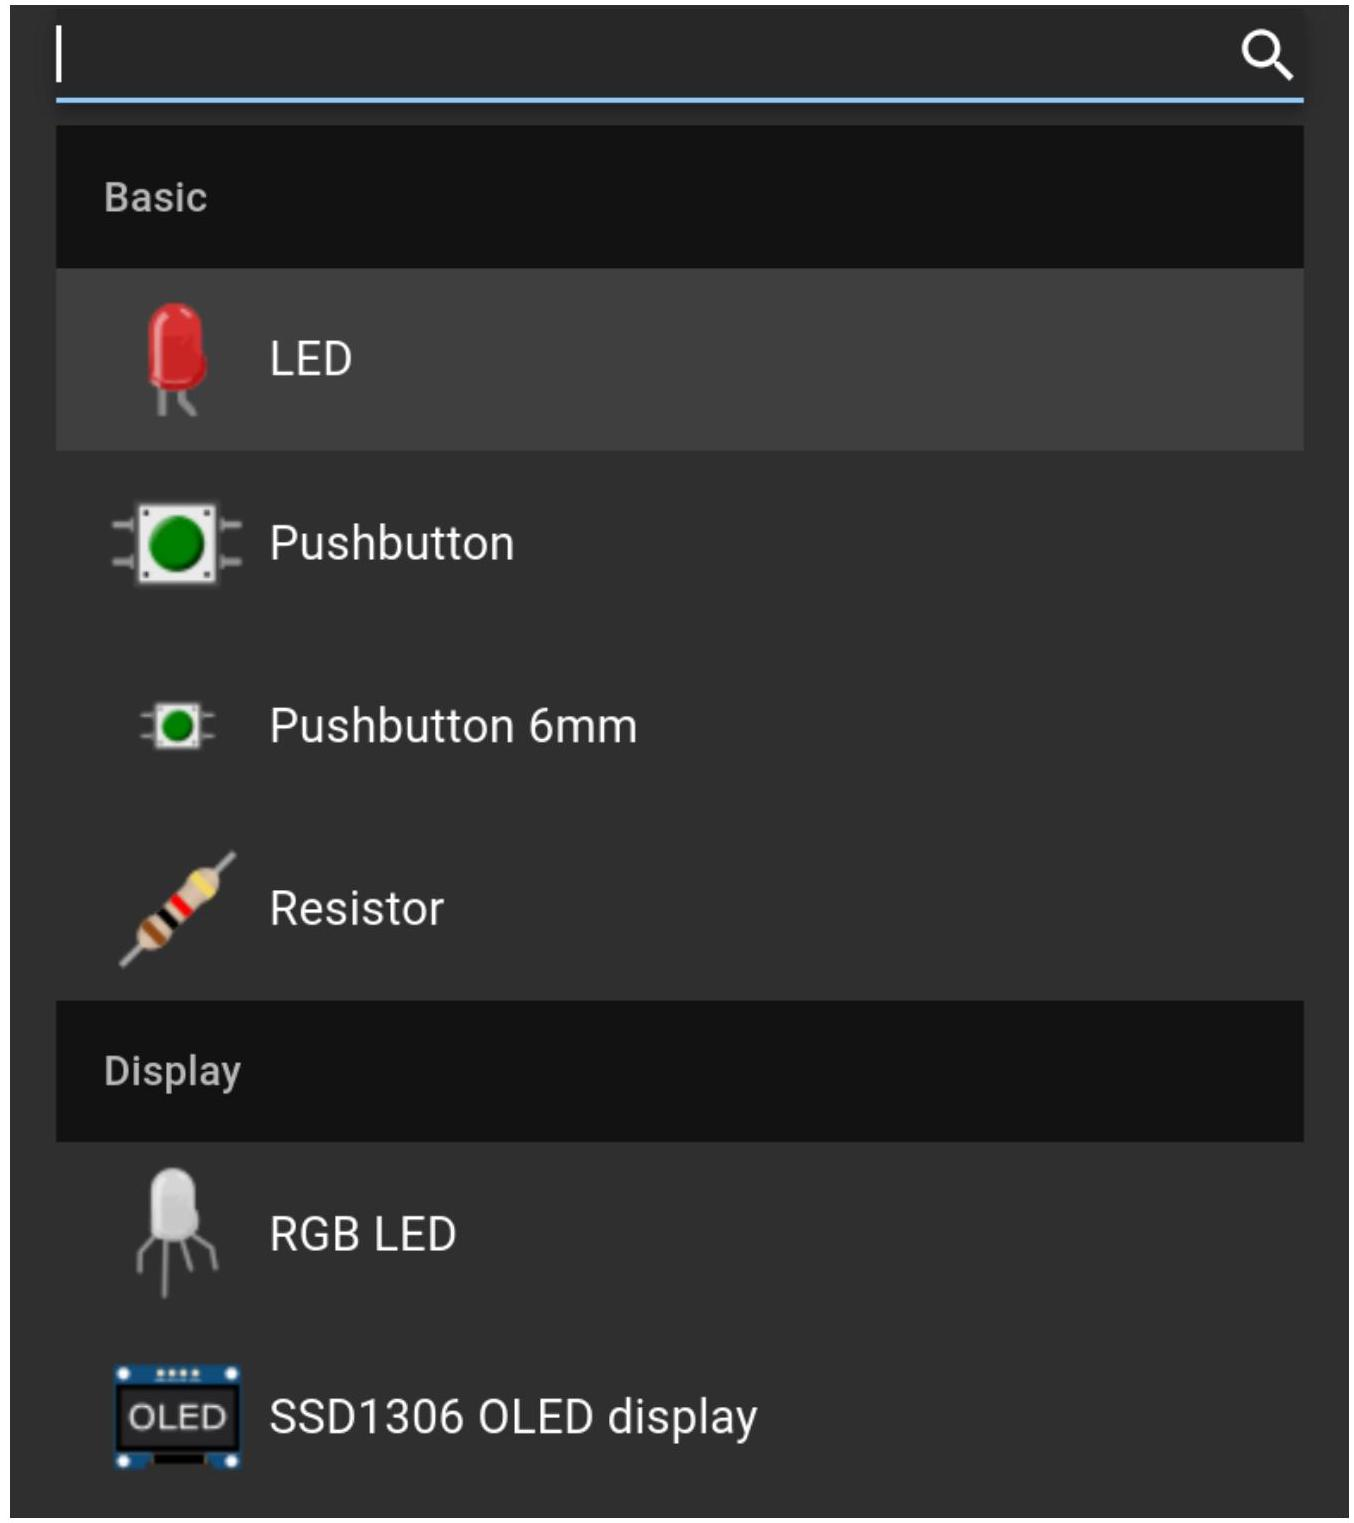
\includegraphics[max width=\maxwidth, max height=\maxheight, center]{11}

\end{enumerate}
% \begin{figure}[htbp]
%     \centering
%     \caption{<caption>}
%     \label{<label>}
% \end{figure}


% \section{План}

% \begin{enumerate}
%     \item Мигание светодиодом. \texttt{delay()}, \texttt{digitalWrite()}
%     \item Маячок с нарастающей яркостью. \texttt{ШИМ}, \texttt{analogWrite()}, Идентификаторы
%     \item Регулируемая лампочка. \texttt{analogRead()}, \texttt{int}, Переменные
%     \item Автоматический ночник. \texttt{bool}, \texttt{if()}
%     \item Пульс. \texttt{mod}
%     \item Бегущий огонь. \texttt{for()}
%     \item Вентилятор. Силовая нагрузка. Мотор
%     \item Световой телеграф. подключение кнопок, \texttt{digitalRead()}
%     \item Лампочка с кнопкой. Защита от дребезга
%     \item Регулируемая лампочка. Функции
%     \item Кнопочные ковбои. Массивы
%     \item Секундомер. Семисегментный индикатор, \texttt{bitRead()}
%     \item Счетчик нажатий. Сдвиговый регистр, \texttt{shiftOut()}
%     \item Комнатный термометр. Датчик температуры. Математические выражения
%     \item Метеостанция. \texttt{Serial.print()}, \texttt{Serial.println()}
%     \item Пантограф. \texttt{Servo}
%     \item USB лампочка. \texttt{Serial.read()}
% \end{enumerate}

\renewcommand{\maxwidth}{0.8\textwidth}
\renewcommand{\maxheight}{0.6\textheight}


% \newcommand{\nametext}{NULL}
% \newcommand{\name}{null}

\newcommand{\listingname}{listing.cpp}
\newcommand{\imagename}{image.jpg}

\newcommand{\illustration}[2]{
\graphicspath{{#1}}

\begin{figure}[!htbp]
    \centering
    \includegraphics[max width=\maxwidth, max height=\maxheight, center]{\imagename}
    \caption{#2}
    \label{#1}
\end{figure}
}

\newcommand{\illustrationlisting}[2]{
\inputminted[linenos]{c++}{#1/\listingname}
}

\newcommand{\task}[2]{

\clearpage
\section{#2}

\illustration{#1}{#2}
\illustrationlisting{#1}{#2}

}



% \task{10_hello_world}{Привет, мир!}

% \illustration{10_hello_world}{HELLO}
% \illustrationlisting{10_hello_world}{HELLO}

\task{10_hello_world}{Привет, мир!}

\task{20_smooth_beacon}{Плавный маяк}

\task{30_adj_light}{Регулируемая лампочка}

\task{40_automatic_night_light}{Автоматический ночник}

\task{50_pulsar}{Пульсар}

\task{60_equalizer}{Эквалайзер}

\task{70_buttons}{Кнопки}

\end{document}